\chapter{\label{ch:ch02}ГЛАВА 2. Разработка игры}

\section{\label{sec:ch02/sec01}Раздел 1. Проектирование игрового процесса и механик}

\subsection{\label{subsec:ch02/sec01/sub01}Подраздел 1. Анализ классической Asteroids и определение основных игровых механик}

Анализ основной игры "Asteroids". Ключевые механики:
\begin{itemize}
    \item Управление игровым кораблем в открытом космосе с возможностью перемещения во всех направлениях.
    \item Разрушение астероидов при помощи снарядов, ведущее к их разделению на более мелкие части.
    \item Опасность столкновения с астероидами и другими объектами на игровом поле, что приводит к потере жизней игрока или поражению.
    \item Система отсчета очков, мотивирующая игрока к достижению новых рекордов и улучшению своих результатов.
\end{itemize}

Новые механики:
\begin{itemize}
    \item Выбор сложности в меню настроек, от сложности зависит количество осколков на которые разделяется астероид, их размер, и количество очков, которое дается за их уничтожение.
    \item Онлайн таблица лидеров в реальном времени, после конца игры можно записать себя в таблицу лидеров под любым именем.
    \item Система бонусов и усилений, которые помогают игроку в сражении с астероидами и увеличивают его шансы на выживание.
    \item Различные визуальные и звуковые эффекты для лучшего игрового опыта.
\end{itemize}


\subsection{\label{subsec:ch02/sec01/sub02}Подраздел 2. Определение целей игры, основных действий игрока и правил игрового процесса}

Основные цели, задачи и правила игры:
\begin{itemize}
    \item Цель игры: выжить как можно дольше, уничтожая астероиды и избегая столкновений с ними и другими объектами.
    \item Основные действия игрока: управление кораблем, стрельба по астероидам, уклонение от опасностей и сбор бонусов.
    \item Правила игрового процесса: игрок начинает игру в центре экрана и пытается набрать максимальное количество очков, избегая столкновений и уничтожая астероиды.
\end{itemize}

\subsection{\label{subsec:ch02/sec01/sub03}Подраздел 3. Создание концепции игры, включая уровни сложности, прогрессию и целевые достижения}

Общая концепция игры "Asteroids", включающая:
\begin{itemize}
    \item Уровни сложности: планируется создание нескольких уровней, каждый из которых будет характеризоваться увеличивающимся количеством и скоростью астероидов, а также другими усложнениями игрового процесса.
    \item Целевые достижения: будут определены определенные цели и достижения, например, достижение определенного количества очков, продержаться определенное время или уничтожить определенное количество астероидов.
\end{itemize}

\section{\label{sec:ch02/sec01}Раздел 2. Проектирование и реализация игрового корабля}

- Разработка внешнего вида игрового корабля с учетом эстетических и функциональных требований
- Создание анимаций для игрового корабля, включая анимацию движения, выстрелов и уничтожения
- Реализация управления игровым кораблем с использованием клавиатуры, мыши или других устройств ввода
- Программирование взаимодействия игрового корабля с окружающим миром, такое как столкновения с астероидами и другими игровыми объектами

\subsection{\label{subsec:ch02/sec01/sub01}Подраздел 1. Разработка внешнего вида игрового корабля}

Корабль представлен простым белым треугольником, сзади которого при движении выпускаются эффекты огня (работы двигателя), стреляет корабль из своего "носа" желтыми круглыми пулями.

\begin{figure}
    \centering
    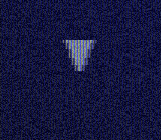
\includegraphics[width=0.5\linewidth]{images/spaceship.png}
    \caption{Космический корабль}
    \label{fig:enter-label}
\end{figure}

\subsection{\label{subsec:ch02/sec01/sub02}Подраздел 2. Реализация управления игровым кораблем}


Реализация управления игровым кораблем в скрипте player.gd~\ref{code:example01}.
\begin{code}
\captionof{listing}{\centering\label{code:example01}Код для движения корабля}
\vspace{-\baselineskip}\begin{minted}{C}
func move(delta):
    # Задаем направление поворота персонажа
    rotation_direction = Input.get_axis("ui_left", "ui_right")
    # Проверяем нажата ли клавиша для движения вперед
    is_moving = Input.is_action_pressed("forward")

    # Поворот персонажа при нажатии клавиш
    if rotation_direction > 0:
        rotation += rotation_speed * delta
    elif rotation_direction < 0:
        rotation -= rotation_speed * delta

    # Если клавиша вперед нажата двигаемся вперед относительно поворота персонажа
    # И замедляемся, при отжатии клавиши
    if is_moving:
        velocity += Vector2(0, 1).rotated(rotation) * speed
    else:
        velocity = velocity.move_toward(Vector2.ZERO, deceleration)
    velocity = velocity.clamp(-max_speed_vector, max_speed_vector)
\end{minted}
\end{code}

Функция "move" находится в основной функции \_physics\_process(delta), которая обновляется каждый кадр, где delta - разность во времени между двумя кадрами.

\subsection{\label{subsec:ch02/sec01/sub03}Подраздел 3. Программирование взаимодействия игрового корабля с окружающим миром}

При столкновении с астероидом конец игры и переход в следующую сцену~\ref{code:example02}.
\begin{code}
\captionof{listing}{\centering\label{code:example02}Код для конца игры}
\vspace{-\baselineskip}\begin{minted}{C}
func _on_collision_player_body_entered(body):
    if body is Enemy:
        die()


func die():
    get_tree().change_scene_to_file("res://Scenes/end_screen.tscn")
\end{minted}
\end{code}


Перемещение персонажа при достижении края экрана~\ref{code:example03}.
\begin{code}
\captionof{listing}{\centering\label{code:example03}Код для перемещения персонажа при достижении края экрана}
\vspace{-\baselineskip}\begin{minted}{C}
func out_of_bounds():
    position = position.posmodv(screen_size)
\end{minted}
\end{code}


Реализация стрельбы при нажатии определенной кнопки и реализация улучшения "тройной выстрел"~\ref{code:example03}.
\begin{code}
\captionof{listing}{\centering\label{code:example03}Код для стрельбы}
\vspace{-\baselineskip}\begin{minted}{C}
func shoot():
    # Уменьшаем таймер пули на 1
    bullet_timer -= 1

    # Если нельзя стрелять и таймер пули меньше или равен 0
    if !can_shoot and bullet_timer <= 0:
        # Разрешаем стрельбу и сбрасываем таймер пули
        can_shoot = true
        bullet_timer = 20

    # Если можно стрелять и нажата кнопка "shoot"
    if can_shoot and Input.is_action_just_pressed("shoot"):
        # Устанавливаем случайный масштаб высоты звука для аудиоплеера и запускаем звук
        $AudioStreamPlayer.pitch_scale = randf_range(0.8, 1.6)
        $AudioStreamPlayer.playing = true

        # Запрещаем стрельбу до следующего разрешения
        can_shoot = false
        # Создаем экземпляр пули из заданного пути
        var bullet = BULLET_PATH.instantiate()

        # Если включен режим тройной стрельбы
        if Globals.triple_shot:
            # Создаем и настраиваем второй экземпляр пули
            var bullet2 = bullet.duplicate()
            bullet2.global_position = $Marker2D.global_position + Vector2(10, 10)
            bullet2.velocity = Vector2(0, 1).rotated(rotation) * bullet_speed
            bullet2.scale = Vector2(0.1, 0.1)
            # Создаем и настраиваем третий экземпляр пули
            var bullet3 = bullet.duplicate()
            bullet3.global_position = $Marker2D.global_position + Vector2(-10, -10)
            bullet3.velocity = Vector2(0, 1).rotated(rotation) * bullet_speed
            bullet3.scale = Vector2(0.1, 0.1)
            # Добавляем вторую и третью пули в родительский узел
            get_parent().add_child(bullet2)
            get_parent().add_child(bullet3)

        # Устанавливаем масштаб пули
        bullet.scale = Vector2(0.1, 0.1)

        # Добавляем пулю в родительский узел
        get_parent().add_child(bullet)
        # Устанавливаем позицию и скорость пули
        bullet.position = $Marker2D.global_position
        bullet.velocity = Vector2(0, 1).rotated(rotation) * bullet_speed

\end{minted}
\end{code}

\subsection{\label{subsec:ch02/sec01/sub02}Подраздел 2. Реализация управления игровым объектом}

Реализация управления игровым объектом в скрипте player.gd~\ref{code:example01}.
\begin{code}
\captionof{listing}{\centering\label{code:example01}Код для управления игровым объектом}
\vspace{-\baselineskip}\begin{minted}{gdscript}
extends CharacterBody2D

var life_timer
var screen_size = Vector2(480, 320)

func _physics_process(_delta):
    out_of_bounds()
    # Обрабатываем движение объекта
    move_and_slide()
    die()

func die():
    # Создаем таймер на 1 секунду
    life_timer = get_tree().create_timer(1, false)
    # Ждем, пока таймер истечет
    await life_timer.timeout
    # Включаем эмиссию частиц
    $CPUParticles2D.emitting = true
    # Скрываем спрайт
    $Sprite2D.hide()

# Проверяем, вышел ли объект за границы экрана
func out_of_bounds():
    # Если объект выходит за границы экрана, перемещаем его на противоположную сторону
    position = position.posmodv(screen_size)

# Удаляем объект, когда анимация частиц закончена
func _on_cpu_particles_2d_finished():
    queue_free()

# Удаляем объект при столкновении с другим объектом
func _on_my_hit_box_area_entered(_area):
    queue_free()

\end{minted}
\end{code}

Функция \_physics\_process выполняет основные операции, обновляемые каждый кадр. Она вызывает три функции: out\_of\_bounds, move\_and\_slide и die, которые описаны ниже.

Функция die отвечает за удаление игрового объекта после одной секунды его существования, а также за активацию эмиссии частиц и скрытие спрайта.

\subsection{\label{subsec:ch02/sec01/sub03}Подраздел 3. Реализация функции удаления объекта}
Реализация функции удаления объекта в скрипте bullet.gd~\ref{code:example02}.
\begin{code}
\captionof{listing}{\centering\label{code:example02}Код для удаления объекта}
\vspace{-\baselineskip}\begin{minted}{gdscript}
func die():
    life_timer = get_tree().create_timer(1, false)
    await life_timer.timeout
    $CPUParticles2D.emitting = true
    $Sprite2D.hide()
\end{minted}
\end{code}

\subsection{\label{subsec:ch02/sec01/sub04}Подраздел 4. Реализация функции контроля границ экрана}
Реализация функции контроля границ экрана в скрипте bullet.gd~\ref{code:example03}.
\begin{code}
\captionof{listing}{\centering\label{code:example03}Код для контроля границ экрана}
\vspace{-\baselineskip}\begin{minted}{gdscript}
func out_of_bounds():
    position = position.posmodv(screen_size)
\end{minted}
\end{code}

Функция out\_of\_bounds использует метод posmodv для циклического переноса позиции объекта в пределах экрана.

\subsection{\label{subsec:ch02/sec01/sub05}Подраздел 5. Реализация функции завершения эмиссии частиц}
Реализация функции завершения эмиссии частиц в скрипте bullet.gd~\ref{code:example04}.
\begin{code}
\captionof{listing}{\centering\label{code:example04}Код для завершения эмиссии частиц}
\vspace{-\baselineskip}\begin{minted}{gdscript}
func _on_cpu_particles_2d_finished():
    queue_free()
\end{minted}
\end{code}

Функция \_on\_cpu\_particles\_2d\_finished вызывается при завершении эмиссии частиц и удаляет объект из сцены, используя метод queue\_free.

\subsection{\label{subsec:ch02/sec01/sub06}Подраздел 6. Реализация функции обработки входа в область хитбокса}
Реализация функции обработки входа в область хитбокса в скрипте bullet.gd~\ref{code:example05}.
\begin{code}
\captionof{listing}{\centering\label{code:example05}Код для обработки входа в область хитбокса}
\vspace{-\baselineskip}\begin{minted}{gdscript}
func _on_my_hit_box_area_entered(_area):
    queue_free()
\end{minted}
\end{code}

Функция \_on\_my\_hit\_box\_area\_entered вызывается при входе другого объекта в хитбокс и удаляет текущий объект, используя метод queue\_free.

\subsection{\label{subsec:ch02/sec01/sub07}Подраздел 7. Скрипт для камеры}
Скрипт для камеры~\ref{code:example06}.
\begin{code}
\captionof{listing}{\centering\label{code:example06}Код для следования камеры за курсором}
\vspace{-\baselineskip}\begin{minted}{gdscript}
extends Camera2D

func _init():
    # Инициализируем позицию камеры в начало координат (0, 0)
    position = Vector2.ZERO

func _input(event : InputEvent) -> void:
    # Проверяем, является ли событие движением мыши
    if event is InputEventMouseMotion:
        # Определяем цель для перемещения камеры, вычитая 10% от размера вьюпорта из позиции курсора
        var _target = event.position - get_viewport().size * 0.1
        # Устанавливаем новую позицию камеры с учетом нормализованного вектора и длины
        self.position = _target.normalized() * (_target.length()) * 0.01


\end{minted}
\end{code}

\subsection{\label{subsec:ch02/sec01/sub08}Подраздел 8. Скрипт для экрана с концом игры}
Скрипт для экрана с концом игры~\ref{code:example07}.
\begin{code}
\captionof{listing}{\centering\label{code:example07}Код для экрана конца игры}
\vspace{-\baselineskip}\begin{minted}{gdscript}
extends Control

@onready var over : RichTextLabel = $RichTextLabel
var speed = 10

func _ready():
    # Устанавливаем текст метки на "SCORE" и текущий счёт из глобальных переменных
    $Label.text = "SCORE %s" % Globals.score
    # Перемещаем фокус на LineEdit для ввода имени игрока
    $LineEdit.grab_focus()

func _process(delta):
    # Вызываем функцию для анимации надписи "Game Over"
    move_game_over(delta)
    # Проверяем, введено ли имя игрока
    if $LineEdit.text == "":
        # Если имя не введено, отключаем кнопку подтверждения
        $Confirm.disabled = true
    else:
        # Если имя введено, сохраняем его в глобальных переменных и активируем кнопку подтверждения
        Globals.player_name = $LineEdit.text
        $Confirm.disabled = false

func move_game_over(delta):
    # Получаем текущую позицию по оси X для надписи "Game Over"
    var current_x = over.position.x
    # Рассчитываем новую позицию с учетом скорости и времени кадра
    var new_x = current_x + speed * delta

    # Проверяем границы движения и изменяем направление при достижении предела
    if new_x < 118:
        new_x = 118
        speed = -speed
    elif new_x > 148:
        new_x = 148
        speed = -speed

    # Устанавливаем новую позицию по оси X для надписи "Game Over"
    over.position.x = new_x

func _on_confirm_pressed():
    # Сохраняем результат игрока и сбрасываем счёт
    SilentWolf.Scores.save_score(Globals.player_name, Globals.score)
    Globals.score = 0
    # Переходим к сцене меню
    get_tree().change_scene_to_file("res://Scenes/menu.tscn")

func _on_restart_pressed():
    # Сбрасываем счёт
    Globals.score = 0
    # Переходим к основной игровой сцене
    get_tree().change_scene_to_file("res://Scenes/main.tscn")


\end{minted}
\end{code}

\label{{subsec:ch02/sec01/sub09}Подраздел 9. Скрипт для астероида}
Скрипт для астероида~\ref{code:example08}.
\begin{code}
\captionof{listing}{\centering\label{code:example08}Код для управления астероидом}
\vspace{-\baselineskip}\begin{minted}{gdscript}

class_name Enemy
extends RigidBody2D

enum asteroid_size {
    LARGE,
    MEDIUM,
    SMALL
}

var mob_scale
var hitpoint : int = 1
var collision_scale
var size
var _explosion_count : int
var shatter_amount : int = 2
@onready var upgrade_scene = preload("res://Scenes/upgrades.tscn")
@onready var audio_player : AudioStreamPlayer = $"../../../Audio/EnemyExplosion"

func _init():
    # Инициализация переменных в зависимости от сложности
    collision_scale = Vector2(0.1, 0.1)
    match Globals.difficulty:
        0:
            _explosion_count = 1
            shatter_amount = 0
            if size == null:
                size = asteroid_size.SMALL
        1:
            _explosion_count = 2
            shatter_amount = 1
            if size == null:
                size = asteroid_size.MEDIUM
        2:
            _explosion_count = 3
            shatter_amount = 2
            if size == null:
                size = asteroid_size.LARGE
    update_size()
    scale = mob_scale

func _physics_process(_delta):
    # Обновление размера и масштаба в каждом кадре
    update_size()
    scale = mob_scale
    $RigidbodyCollision.scale = collision_scale

func take_damage(amount: int):
    # Уменьшаем количество хитпоинтов на заданное значение
    hitpoint -= amount
    # Если хитпоинты закончились
    if hitpoint <= 0:
        spawn_random_upgrade()
        # Проверяем размер астероида и выполняем соответствующие действия
        if size == asteroid_size.LARGE:
            Globals.score += 1
            explode(0)
            hitpoint = 1
        elif size == asteroid_size.MEDIUM:
            Globals.score += 2
            explode(1)
            hitpoint = 1
        else:
            Globals.score += 3
            $CPUParticles2D.emitting = true
            $Rock.hide()
            $Trail.hide()
    update_size()

func _on_cpu_particles_2d_finished():
    # Удаляем объект, когда частицы завершили эмиссию
    queue_free()

func update_size():
    # Обновление масштаба в зависимости от размера астероида
    match size:
        asteroid_size.LARGE:
            mob_scale = Vector2(5, 5)
        asteroid_size.MEDIUM:
            mob_scale = Vector2(3.5, 3.5)
        asteroid_size.SMALL:
            mob_scale = Vector2(2, 2)

func explode(current_size : int):
    # Логика взрыва астероида и создания новых меньших астероидов
    var explosion_count = _explosion_count
    audio_player.pitch_scale = randf_range(0.8, 1.3)
    audio_player.playing = true
    queue_free()
    if current_size == 0:
        for i in range(explosion_count):
            var new_asteroid = duplicate()
            new_asteroid.size = asteroid_size.MEDIUM
            new_asteroid.global_position = global_position + Vector2(randf_range(-25, 25), randf_range(-25, 25))
            new_asteroid.shatter_amount = 1
            new_asteroid.linear_velocity = Vector2(randf_range(-175, 175), randf_range(-175, 175))
            get_parent().add_child(new_asteroid)
    elif current_size == 1:
        for i in range(explosion_count):
            var new_asteroid = duplicate()
            new_asteroid.size = asteroid_size.SMALL
            new_asteroid.global_position = global_position + Vector2(randf_range(-25, 25), randf_range(-25, 25))
            new_asteroid.shatter_amount = 0
            new_asteroid.linear_velocity = Vector2(randf_range(-175, 175), randf_range(-175, 175))
            get_parent().add_child(new_asteroid)

func _on_visible_on_screen_notifier_2d_screen_exited():
    # Удаляем объект, когда он выходит за границы экрана
    queue_free()

func spawn_random_upgrade():
    # Случайным образом создаем апгрейд
    var random_drop_chance = randf_range(0,100)
    var random_upgrade_spawn = randf_range(0,100)
    if int(random_drop_chance) <= 10:
        var upg = upgrade_scene.instantiate()
        upg.global_position = global_position
        var rand_upg = upg.find_child("AnimatedSprite2D")
        if random_upgrade_spawn <= 50:
            rand_upg.play("time_stop")
        else:
            rand_upg.play("triple_shot")
        get_parent().add_child(upg)


\end{minted}
\end{code}

\label{{subsec:ch02/sec01/sub10}Подраздел 10. Скрипт для частиц двигателя}
Скрипт для частиц двигателя~\ref{code:example09}.
\begin{code}
\captionof{listing}{\centering\label{code:example09}Код для частиц двигателя}
\vspace{-\baselineskip}\begin{minted}{gdscript}

extends CPUParticles2D

@onready var player = $".."
var max_velocity : int = 55

func _ready():
    # Скрываем частицы при инициализации
    hide()

func _physics_process(_delta):
    # Проверяем, движется ли игрок
    if player.velocity != Vector2.ZERO:
        # Постепенно увеличиваем максимальную скорость до 55
        max_velocity = move_toward(max_velocity, 55, 5)
        # Устанавливаем максимальную начальную скорость для частиц
        initial_velocity_max = max_velocity
        # Показываем частицы
        show()
    else:
        # Постепенно уменьшаем максимальную скорость до 0
        max_velocity = move_toward(max_velocity, 0, 1)
        # Устанавливаем максимальную начальную скорость для частиц
        initial_velocity_max = max_velocity
        # Скрываем частицы, если скорость практически равна нулю
        if initial_velocity_max <= 1:
            hide()
    # Устанавливаем направление силы тяжести противоположное направлению движения игрока
    gravity = -Vector2(0, 1).rotated(rotation) * 100


\end{minted}
\end{code}

\label{{subsec:ch02/sec01/sub11}Подраздел 11. Скрипт для глобальных переменных и api таблицы лидеров}
Скрипт для глобальных переменных и api таблицы лидеров~\ref{code:example10}.
\begin{code}
\captionof{listing}{\centering\label{code:example10}Код для глобальных переменных и api таблицы лидеров}
\vspace{-\baselineskip}\begin{minted}{gdscript}
extends Node

var score : int = 0
var player_name : String
var last_scene_path : String
var difficulty : int = 1
var triple_shot : bool = false

# Sounds volume
var master_volume : int = 5
var music_volume : int = 5
var sfx_volume : int = 5

func _ready():
    SilentWolf.configure({
        "api_key": "",
        "game_id": "asteroids",
        "log_level": 0
    })

    SilentWolf.configure_scores({
        "open_scene_on_close": "res://Scenes/menu.tscn"
    })

\end{minted}
\end{code}

\label{{subsec:ch02/sec01/sub12}Подраздел 12. Скрипт для получения урона}
Скрипт для получения урона~\ref{code:example11}.
\begin{code}
\captionof{listing}{\centering\label{code:example11}Код для получения урона}
\vspace{-\baselineskip}\begin{minted}{gdscript}

class_name MyHurtBox
extends Area2D

func _init() -> void:
    # Устанавливаем слой и маску столкновения
    collision_layer = 2
    collision_mask = 2


func _ready() -> void:
    # Подключаем сигнал "area_entered" к методу "_on_area_entered"
    connect("area_entered", self._on_area_entered)


func _on_area_entered(hitbox: MyHitBox):
    # Проверяем, не является ли hitbox нулевым значением
    if hitbox == null:
        return

    # Если у владельца есть метод "take_damage", вызываем его с параметром "damage" из hitbox
    if owner.has_method("take_damage"):
        owner.take_damage(hitbox.damage)


\end{minted}
\end{code}

\label{{subsec:ch02/sec01/sub13}Подраздел 13. Скрипт для интерфейса в процессе игры}
Скрипт для интерфейса в процессе игры~\ref{code:example12}.
\begin{code}
\captionof{listing}{\centering\label{code:example12}Код для интерфейса в процессе игры}
\vspace{-\baselineskip}\begin{minted}{gdscript}
extends Node

func _ready():
    # Устанавливаем начальные значения глобальных переменных
    Globals.last_scene_path = "res://Scenes/main.tscn"
    Globals.triple_shot = false
    Globals.score = 0
    # Снимаем паузу с игрового дерева
    get_tree().paused = false


func _process(delta):
    # Проверяем, была ли нажата кнопка паузы
    if Input.is_action_just_pressed("pause"):
        _on_menu_button_pressed()


func _on_menu_button_pressed():
    # Воспроизводим звук нажатия кнопки
    $Audio/Click.playing = true
    ## Пауза при нажатии кнопки
    match get_tree().paused:
        true:
            # Если игра на паузе, создаем таймер на 0.2 секунды, ждем его завершения и снимаем паузу
            var pause_timer = get_tree().create_timer(0.2)
            await pause_timer.timeout
            get_tree().paused = false
        false:
            # Если игра не на паузе, ставим на паузу и переходим на сцену с опциями
            get_tree().paused = true
            get_tree().change_scene_to_file("res://Scenes/options.tscn")


func _on_back_ground_music_finished():
    # При окончании музыки запускаем ее заново
    $Audio/BackGroundMusic.playing

\end{minted}
\end{code}

\label{{subsec:ch02/sec01/sub14}Подраздел 14. Скрипт для появления "врагов" и обновления счета}
Скрипт для появления "врагов" и обновления счета~\ref{code:example13}.
\begin{code}
\captionof{listing}{\centering\label{code:example13}Код для появления "врагов" и обновления счета}
\vspace{-\baselineskip}\begin{minted}{gdscript}
extends SubViewport

@export var mob_scene: PackedScene
@export var max_asteroid_velocity : float = 175.0
@onready var asteroids = $Enemy
@onready var score_label = $"../../UI/Score"

func _process(delta):
    # Обновляет отображение счета каждый кадр
    score_update()


func _on_mob_timer_timeout():
    # Создаем новый экземпляр астероида
    var mob = mob_scene.instantiate()

    # Определяем местоположение для появления астероида
    var mob_spawn_location = $MobPath/MobSpawnLocation
    mob_spawn_location.progress_ratio = randf()

    # Задаем направление движения астероида
    var direction = mob_spawn_location.rotation + PI/2

    # Устанавливаем позицию астероида в точку появления
    mob.position = mob_spawn_location.position

    # Добавляем случайное отклонение к направлению
    direction += randf_range(-PI/4, PI/4)
    mob.rotation = direction

    # Задаем скорость астероида
    var velocity = Vector2(randf_range(max_asteroid_velocity - 100, max_asteroid_velocity), 0.0)
    mob.linear_velocity = velocity.rotated(direction)
    mob.get_child(2).gravity = velocity

    # Добавляем астероид в сцену
    add_child(mob)


func score_update():
    # Обновляем текст метки счета
    score_label.text = "%s" % Globals.score

\end{minted}
\end{code}

\label{{subsec:ch02/sec01/sub15}Подраздел 15. Скрипт для api таблицы лидеров}
Скрипт для api таблицы лидеров~\ref{code:example14}.
\begin{code}
\captionof{listing}{\centering\label{code:example14}Код для api таблицы лидеров}
\vspace{-\baselineskip}\begin{minted}{gdscript}

extends Control

# Загружаем сцену элемента счета
const ScoreItem = preload("res://addons/silent_wolf/Scores/ScoreItem.tscn")
# Загружаем скрипт утилиты Silent Wolf Logger
const SWLogger = preload("res://addons/silent_wolf/utils/SWLogger.gd")

# Индекс списка
var list_index = 0
# Название таблицы лидеров, если вы не используете таблицу лидеров по умолчанию
var ld_name = "main"
# Максимальное количество отображаемых счетов
var max_scores = 10

func _ready():
    # Устанавливаем путь к последней сцене
    Globals.last_scene_path = "res://Scenes/menu.tscn"
    # Устанавливаем фокус на кнопку "Start"
    $VBoxContainer/Start.grab_focus()

    #region Лидерборд API
    # Получаем данные о счетах из хранилища
    var scores = SilentWolf.Scores.scores
    #var scores = []
    # Если указанное имя лидерборда есть в списке лидербордов, используем его данные
    if ld_name in SilentWolf.Scores.leaderboards:
        scores = SilentWolf.Scores.leaderboards[ld_name]
    # Получаем локальные счета
    var local_scores = SilentWolf.Scores.local_scores

    # Если есть какие-то данные о счетах, отображаем их
    if len(scores) > 0:
        render_board(scores, local_scores)
    else:
        # Иначе загружаем данные о счетах, пока не будут получены данные, показывая "loading" анимацию...
        add_loading_scores_message()
        var sw_result = await SilentWolf.Scores.get_scores().sw_get_scores_complete
        scores = sw_result.scores
        hide_message()
        render_board(scores, local_scores)
    #endregion

# Отображает данные о счетах
func render_board(scores: Array, local_scores: Array) -> void:
    var all_scores = scores
    # Если используется таблица лидерборда по умолчанию, объединяем данные о счетах с локальными
    if ld_name in SilentWolf.Scores.ldboard_config and is_default_leaderboard(SilentWolf.Scores.ldboard_config[ld_name]):
        all_scores = merge_scores_with_local_scores(scores, local_scores, max_scores)
        if scores.is_empty() and local_scores.is_empty():
            add_no_scores_message()
    else:
        if scores.is_empty():
            add_no_scores_message()
    if all_scores.is_empty():
        for score in scores:
            add_item(score.player_name, str(int(score.score)))
    else:
        for score in all_scores:
            add_item(score.player_name, str(int(score.score)))

# Проверяет, является ли таблица лидерборда таблицей по умолчанию
func is_default_leaderboard(ld_config: Dictionary) -> bool:
    var default_insert_opt = (ld_config.insert_opt == "keep")
    var not_time_based = !("time_based" in ld_config)
    return default_insert_opt and not_time_based

# Объединяет данные о счетах с локальными данными
func merge_scores_with_local_scores(scores: Array, local_scores: Array, max_scores: int=10) -> Array:
    if local_scores:
        for score in local_scores:
            var in_array = score_in_score_array(scores, score)
            if !in_array:
                scores.append(score)
            scores.sort_custom(sort_by_score)
    if scores.size() > max_scores:
        var new_size = scores.resize(max_scores)
    return scores

# Сортирует данные о счетах по счету
func sort_by_score(a: Dictionary, b: Dictionary) -> bool:
    if a.score > b.score:
        return true
    else:
        if a.score < b.score:
            return false
        else:
            return true

# Проверяет, содержится ли данный счет в массиве счетов
func score_in_score_array(scores: Array, new_score: Dictionary) -> bool:
    var in_score_array =  false
    if !new_score.is_empty() and !scores.is_empty():
        for score in scores:
            if score.score_id == new_score.score_id:
                in_score_array = true
    return in_score_array

# Добавляет элемент счета
func add_item(player_name: String, score_value: String) -> void:
    pass

# Добавляет сообщение о том, что счетов нет
func add_no_scores_message() -> void:
    pass

# Добавляет сообщение о загрузке счетов
func add_loading_scores_message() -> void:
    pass

# Скрывает сообщение
func hide_message() -> void:
    pass

# Очищает лидерборд
func clear_leaderboard() -> void:
    pass
#endregion


# Обработчики событий кнопок

func _on_start_pressed():
    get_tree().change_scene_to_file("res://Scenes/main.tscn")


func _on_quit_pressed():
    get_tree().quit()


func _on_leaderboard_pressed():
    get_tree().change_scene_to_file("res://Scenes/leaderboard.tscn")


func _on_options_pressed():
    get_tree().change_scene_to_file("res://Scenes/options.tscn")



\end{minted}
\end{code}

\label{{subsec:ch02/sec01/sub16}Подраздел 16. Скрипт для настроек}
Скрипт для настроек~\ref{code:example15}.
\begin{code}
\captionof{listing}{\centering\label{code:example15}Код для настроек}
\vspace{-\baselineskip}\begin{minted}{gdscript}

extends Control

# Ссылка на элемент OptionButton, отвечающий за выбор сложности
@onready var difficulty : OptionButton = $VBoxContainer/HBoxContainer/OptionButton

func _ready():
    # Если последняя сцена была главной игровой сценой, отключаем выбор сложности
    if Globals.last_scene_path == "res://Scenes/main.tscn":
        difficulty.disabled = true
    # Устанавливаем фокус на кнопку "Back"
    $Back.grab_focus()
    # Добавляем пункты выбора сложности в OptionButton
    difficulty.add_item("EASY", 0)
    difficulty.add_item("NORMAL", 1)
    difficulty.add_item("HARD", 2)
    # Устанавливаем выбранную сложность в соответствии с глобальной переменной
    difficulty.select(Globals.difficulty)

# Обработчик события нажатия кнопки "Back"
func _on_back_pressed():
    # Проверяем последнюю сцену и возвращаемся на соответствующую сцену
    match Globals.last_scene_path:
        "res://Scenes/menu.tscn":
            get_tree().change_scene_to_file("res://Scenes/menu.tscn")
        "res://Scenes/main.tscn":
            get_tree().change_scene_to_file("res://Scenes/main.tscn")

# Обработчик события выбора пункта в OptionButton для выбора сложности
func _on_option_button_item_selected(index):
    # Обновляем глобальную переменную, представляющую выбранную сложность
    Globals.difficulty = index

# Обработчик события нажатия кнопки "Credits/Help"
func _on_credits__help_pressed():
    # Переходим на сцену справки
    get_tree().change_scene_to_file("res://Scenes/help.tscn")

\end{minted}
\end{code}

\label{{subsec:ch02/sec01/sub17}Подраздел 17. Скрипт для улучшений}
Скрипт для улучшений~\ref{code:example16}.
\begin{code}
\captionof{listing}{\centering\label{code:example16}Код для улучшений}
\vspace{-\baselineskip}\begin{minted}{gdscript}
class_name Upgrade
extends Node2D

# Таймер остановки времени
@onready var time_stop_timer = $TimeStopTimer

# Функция _ready() вызывается при готовности узла
func _ready():
    # Создаем таймер жизни для апгрейда, после истечения которого апгрейд исчезает
    var life_timer = get_tree().create_timer(5)
    await life_timer.timeout
    # Если апгрейд не скрыт, вызываем функцию уничтожения
    if !hidden:
        die()

# Функция _on_area_2d_area_entered() вызывается при входе в зону обнаружения другого узла
func _on_area_2d_area_entered(area):
    # Если игрок вошел в зону и апгрейд "Time Stop" неактивен, запускаем его
    if area.name == "CollisionPlayer" and $AnimatedSprite2D.get_animation() == "time_stop" and Globals.triple_shot == false and get_tree().paused == false:
        get_tree().paused = true
        $TimeStopTimer.start()
        hide()
        $Area2D.hide()
    # Если игрок вошел в зону и апгрейд "Triple Shot" неактивен, запускаем его
    if area.name == "CollisionPlayer" and $AnimatedSprite2D.get_animation() == "triple_shot" and Globals.triple_shot == false and get_tree().paused == false:
        $TripleShotTimer.start()
        Globals.triple_shot = true
        hide()
        $Area2D.hide()

# Обработчик события истечения времени апгрейда "Time Stop"
func _on_time_stop_timer_timeout():
    # Возобновляем игру
    get_tree().paused = false
    queue_free()

# Обработчик события истечения времени апгрейда "Triple Shot"
func _on_triple_shot_timer_timeout():
    # Сбрасываем статус "Triple Shot"
    Globals.triple_shot = false
    queue_free()

# Функция для удаления апгрейда
func die():
    queue_free()

\end{minted}
\end{code}

\label{{subsec:ch02/sec01/sub19}Подраздел 19. Скрипт для слайдера громкости}
Скрипт для слайдера громкости~\ref{code:example18}.
\begin{code}
\captionof{listing}{\centering\label{code:example18}Код для слайдера громкости}
\vspace{-\baselineskip}\begin{minted}{gdscript}
extends HSlider

# Имя аудио-шины, которую управляет этот ползунок
@export
var bus_name : String

# Индекс аудио-шины
var bus_index : int

func _ready():
    # Устанавливаем текущее значение ползунка равным глобальной переменной уровня громкости мастера
    value = Globals.master_volume
    # Вызываем функцию для обновления громкости аудио-шины
    _on_value_changed(Globals.master_volume)
    bus_index = AudioServer.get_bus_index(bus_name)
    # Подключаем сигнал value_changed к функции _on_value_changed
    value_changed.connect(_on_value_changed)

# Функция _on_value_changed вызывается при изменении значения ползунка
func _on_value_changed(value : float) -> void:
    # Устанавливаем громкость аудио-шины в соответствии с новым значением ползунка
    AudioServer.set_bus_volume_db(
        bus_index,
        linear_to_db(value/10)
    )
    # Обновляем глобальную переменную уровня громкости
    Globals.master_volume = value


\end{minted}
\end{code}

\section{\label{sec:ch02/sec03}Раздел 3. Добавление звуковых эффектов и музыки}

\begin{itemize}
    \item Подбор и добавление звуковых эффектов для различных игровых событий, таких как выстрелы, взрывы и столкновения с помощью сайта \cite{https://sfxr.me/}
    \item Интеграция фоновой музыки для создания атмосферы игры и поддержания интереса игрока. Фоновая музыка (с разрешения автора) \cite{https://www.youtube.com/watch?v=-35AC-FPoAA}
    \item Настройка звуковых уведомлений и звуковых сигналов для обратной связи с пользователем, также с помощью сайта \cite{https://sfxr.me/}
\end{itemize}
 